\documentclass[11pt]{article}
% Кодировка и язык
\usepackage[utf8]{inputenc}           % Кодировка исходного файла (UTF-8)
\usepackage[T2A]{fontenc}             % Кодировка шрифтов для кириллицы
\usepackage[english,russian]{babel}   % Локализация: русские названия, переносы

% Поиск в PDF
\usepackage{cmap}                     

% Поля страницы
\usepackage{geometry}
\geometry{left=2cm, right=2cm, top=2cm, bottom=2cm}

% Математика
\usepackage{amsmath, amssymb, amsthm} % Базовые пакеты для математики
\usepackage{mathtools}                % Расширение amsmath (доп. символы и окружения)

% Картинки
\usepackage{graphicx}                 % Вставка картинок (\includegraphics)
\graphicspath{{pictures/}}            % Путь к папке с картинками
\usepackage{float}                    % Позволяет использовать [H] для жёсткого позиционирования
\usepackage{wrapfig}                  % Обтекание текста вокруг картинок

% Таблицы
\usepackage{array}                    % Расширенные возможности для таблиц
\usepackage{booktabs}                 % Красивые таблицы (\toprule, \midrule, \bottomrule)
\usepackage{multirow}                 % Объединение строк в таблицах
\usepackage{tabularx}                 % Таблицы с автоматической шириной колонок
\usepackage{ragged2e}                 % Улучшенное выравнивание (используется в tabularx)

% Списки
\usepackage{enumitem}                 % Гибкая настройка списков (itemize, enumerate)

% Колонтитулы
\usepackage{fancyhdr}                 

% Гиперссылки
\usepackage{xcolor}                   % Работа с цветами
\usepackage{hyperref}                 % Гиперссылки, оглавление, перекрёстные ссылки

% Умные ссылки
\usepackage{cleveref}                 

% Типографика
\usepackage{microtype}                % Улучшает переносы и межсловные расстояния

% Подписи к картинкам и таблицам
\usepackage{caption}                  % Настройка подписей (шрифт, отступы)

% Рисование схем и графиков
\usepackage{tikz}                     % Рисование схем, графиков, диаграмм
\usepackage{pgfplots}                 % Построение графиков функций (на основе tikz)
\pgfplotsset{compat=newest}           % Версия совместимости pgfplots

% Алгоритмы и код
\usepackage{algorithm}                % Окружения для алгоритмов
\usepackage{algorithmic}              % Синтаксис для алгоритмов
\usepackage{listings}                 % Вставка кода с подсветкой синтаксиса


% Настройка нумерации секций и подсекций
\renewcommand{\thesection}{\arabic{section}}                   
\renewcommand{\thesubsection}{\thesection.\arabic{subsection}} 


% Настройка списков: убираем лишние отступы слева
\setlist[itemize]{leftmargin=}
\setlist[enumerate]{leftmargin=}


% Определение окружений для теорем, лемм, определений и т.д.
% Нумерация привязана к номеру секции
\newtheorem{theorem}{Теорема}[section]
\newtheorem{definition}{Определение}[section]
\newtheorem{remark}{Замечание}[section]
\newtheorem{lemma}{Лемма}[section]
\newtheorem{example}{Пример}[section]
\newtheorem{consequence}{Следствие}[section]
\newtheorem{algorithmm}{Алгоритм}
\newtheorem{question}{Вопрос}[section]
\newtheorem{answer}{Ответ}[section]
\newtheorem{statement}{Утверждение}[section]


% Определение цветов
\definecolor{pblue}{rgb}{0.13,0.13,1}    
\definecolor{pgreen}{rgb}{0,0.5,0}       
\definecolor{pred}{rgb}{0.9,0,0}         
\definecolor{pgrey}{rgb}{0.46,0.45,0.48}
\usetikzlibrary{positioning, arrows.meta}

\newcommand{\lectureNumber}{4}
\newcommand{\lectureTitle}{Полиномиальная схема. Случайные величины. Математическое ожидание}
\newcommand{\courseName}{Теория вероятностей}
\newcommand{\semester}{3 семестр, 2026/2027 уч. год}

\pagestyle{fancy}
\fancyhf{}
\fancyhead[L]{Цветы и пчёлы неразрывны, как выходные и... домашка}
\fancyhead[R]{\thepage}
\setlength{\headheight}{15pt}

\hypersetup{
    colorlinks=true,
    linkcolor=blue!70!black,
    citecolor=blue!70!black,
    filecolor=blue!70!black,
    urlcolor=blue!70!black,
}

\begin{document}


\begin{titlepage}
    \centering
    
    {\large Московский физико-технический институт \par}
    {\large Высшая школа программной инженерии \par}
    \vspace{2cm}

    {\Large \textbf{\courseName} \par}
    {\large \semester \par}
    
    \vspace*{\fill}

    {\Huge \textbf{Лекция \lectureNumber} \par}
    {\Huge \textbf{\lectureTitle} \par}
    
    \vspace*{\fill}
    
    {\large Лектор: Широков М.Е. <3\par}
    {\large Автор: \href{t.me/sol_m_07}{Соля} \par}

\end{titlepage}

\pagenumbering{arabic}

\section{Полиномиальная схема}

\subsection{Биномиальная схема (схема Бернулли)}

Схема испытаний Бернулли заключается в том, что проводятся $n$ испытаний с двумя исходами (условно говоря 1 и 0) с вероятностями $p$ и $q$ соответственно.
Тогда вероятность того, что у нас будет ровно $k$ успехов (единиц) составит
\[C_n^k \cdot p^k \cdot q^{n - k}\]
В этом случае $\Omega = \{0, 1\}$, \ $\widehat{\Omega} = \Omega^{\times n}$, \ $\widehat{\omega} = (x_1, x_2, \ldots, x_n)$, где $x_i \in \{0, 1\}$.

\subsection{Полиномиальная схема}

Своего рода обобщением биномиальной схемы является полиномиальная схема. Представим, что испытаний всё так же $n$, а исходов теперь $m$:
\[A_1, A_2, \ldots, A_m\]
У каждого из них есть своя вероятность $p_i$ и $\displaystyle \sum_{k = 1}^{m} p_k = 1$. \\
Тогда $\Omega = \{A_1, A_2, \ldots, A_m\}$, \ $\widehat{\Omega} = \Omega^{\times n}$, \ $\widehat{\omega} = (x_1, x_2, \ldots, x_n)$, где $x_i \in \{A_1, A_2, \ldots, A_m\}$. \\
Пусть $k_i$ --- количество выпадений $A_i$, при этом конечно же $\displaystyle \sum_{i = 1}^{m} k_i = n$. Тогда
\[\widehat{P} = P(\widehat{\omega}) = \prod_{i = 1}^{m} p_i^{k_i}\]
Считая вероятность выпадения конкретных $k_i$ (количеств $A_i$ в $\widehat{\omega}$) подобно $k$ успехам в пункте 1.1, получим
\[P(k_1, k_2, \ldots, k_m) = [\text{все события с совпадающими $k_i$ равновероятны}] = K \cdot \prod_{i = 1}^{m} p_i^{k_i},\]
где $K = \displaystyle \frac{n!}{k_1! \cdot k_2! \cdot \ldots \cdot k_m!}$ --- полиномиальный коэффициент. \\ \\
\begin{figure}[H]
  \centering
  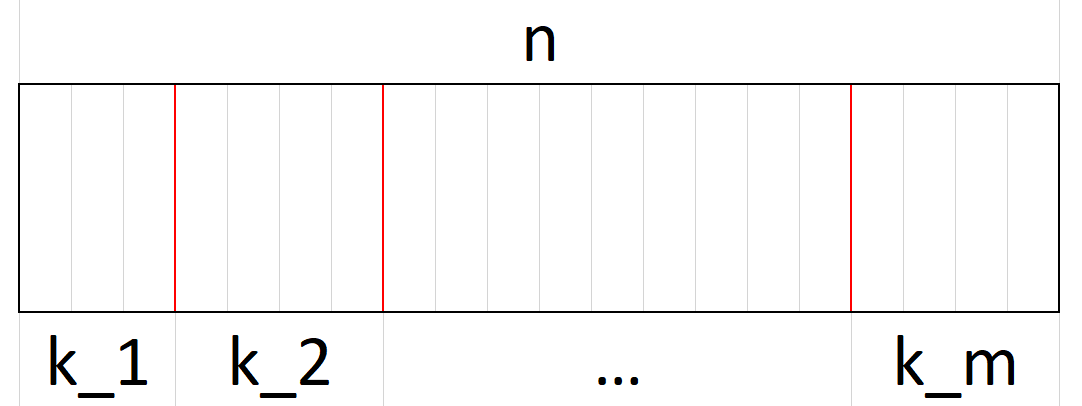
\includegraphics[width=0.7\linewidth]{Полиномиальный коэффициент.png}
\end{figure} \leavevmode
\\
Как его вывести? Представляем полоску на $n$ ячеек. Резервируем от начала последовательно $k_1$ из них, потом $k_2$ и т.д.. 
Всего способов организовать полоску $n!$, но в рамках каждого $i$-го блока перестановка не будет менять сути, так как порядок не важен, а перестановок $k_i!$. Итоговая формула теперь очевидна.

\section{Случайные величины}

Вспомним наше ВП $\Omega = \{\omega_1, \ldots, \omega_N\}$ и рулетку. Она выдаёт какое-то одно $\omega_i$ и мы радуемся. 
Так вот теперь радостью всё не ограничится. После запустим ``постпроцессинг'' и получим $\xi (\omega_i)$, где $\xi \colon \Omega \to \mathbb{R}$.

\begin{definition}
    \textbf{Случайная величина} --- это \underline{любая} вещественнозначная функция на $\Omega$.
\end{definition}

\begin{remark}
    На самом деле случайная величина в общем определяется несколько по-другому (добавляется условие на $\mathcal{F}$-измеримость относительно $\sigma$-алгебры событий), 
    но мы пока что рассматриваем только дискретный случай, а в нём это условие выполняется автоматически.
\end{remark}

\begin{definition}
    Функция на дискретном множестве будет описываться таблицей соответствий (возможно бесконечной):
    \begin{table}[h]
    \centering
    \begin{tabular}{|c|c|c|c|c|}
    \hline
    $\omega_1$ & $\omega_2$ & \ldots & $\omega_i$ & \ldots \\
    \hline
    $\xi(\omega_1)$ & $\xi(\omega_2)$ & \ldots & $\xi(\omega_i)$ & \ldots \\
    \hline
    \end{tabular}
    \end{table}
\end{definition}

\begin{remark}
    Греческие буквы мы будем использовать для случайных величин, а латинские --- для их значений $(\xi(\omega) = x)$. 
    В целом, можно воспринимать это как дань уважения грекам. Давным-давно колоссальный рывок был сделан именно ими, но потом римляне --- грубые тупые мужики, ``мужланы'' --- пришли, завоевали Грецию, всё забрали у них...
\end{remark} \leavevmode
\\
Так как наша функция $\xi$ определена на конечном или счётном множестве, то множество её значений $\xi(\Omega)$ также будет конечным или счётным:
\[\xi \ \sim \ (x_1, x_2, \ldots, x_m), \text{ где для удобства упорядочим } x_1 < x_2 < \ldots < x_m\]
Получим $m < N$ ($N$ --- число исходов в $\Omega$). Можно представлять себе в голове картинку: \\
\begin{center}
\begin{tikzpicture}[
    leftnode/.style={circle, draw, fill=blue!20, minimum size=8mm, inner sep=0pt},
    rightnode/.style={circle, draw, fill=red!20, minimum size=8mm, inner sep=0pt},
    edge/.style={-{Stealth[length=3mm]}, thick}
]

% Левая доля (5 вершин)
\foreach \i in {1,...,5} {
    \node[leftnode] (L\i) at (0, -\i) {$\omega_{\i}$};
}

% Правая доля (3 вершины) — меньше, чтобы была сюръекция
\foreach \i in {1,...,3} {
    \node[rightnode] (R\i) at (4, -1.5*\i - 0.5) {$x_{\i}$};
}

% Стрелки: из каждой левой ровно одна, каждая правая достигается
\draw[edge] (L1) -- (R2);
\draw[edge] (L2) -- (R1);
\draw[edge] (L3) -- (R1);
\draw[edge] (L4) -- (R2);
\draw[edge] (L5) -- (R3);

\end{tikzpicture}
\end{center} \leavevmode
\\
Здесь $5 > 3 \implies$ найдётся хотя бы одно значение $x_i$, которому соответствует несколько $\omega_j$. 
Если бы $m$ и $N$ совпали, то мы бы получили биекцию и $\xi$ была бы обратимой. \\ \\
Определим же вероятность обращения $\xi$ в $x_k$:
\[P_{\xi}(k) \ := \ P(\xi = x_k) \ = \sum_{i: \ \xi(\omega(x_i)) = x_k} P(\omega_i) \ = \sum_{i: \ \xi(\omega(x_i)) = x_k} p_i\]
Обозначение $P_{\xi}(k)$ корректно, так как мы заранее упорядочили $x_i$ и $k$ однозначно нам определяет $x$. Выходит, что $\Omega$ и $\xi$ 
породили новое вероятностное пространство $\mathbb{X}$ (так и будем называть --- пространство, порождённое случайной величиной), где 
конечно же выполнено условие нормировки:
\[\sum_{k = 1}^{m} P_{\xi}(k) = 1\]

\begin{definition}
    Набор чисел $\overline{P}_{\xi} = (P_{\xi}(1), P_{\xi}(2), \ldots, P_{\xi}(m))$ называется \textbf{распределением случайной величины} $\xi$.
\end{definition}

\begin{example}
    Бросаем две симметричные монеты. $\Omega = \{\text{ГГ, ГР, РГ, РР}\}$. Вероятность каждого исхода равна $\frac{1}{4}$. 
    Пусть $\xi$ --- количество гербов. Для распределения нарисуем таблицу:
    \renewcommand{\arraystretch}{2.2}
    \begin{table}[h]
    \centering
    \begin{tabular}{|*{4}{>{\centering\arraybackslash}m{2cm}|}}
    \hline
    $x_i$            & $0$ & $1$ & $2$ \\
    \hline
    $P_{\xi} (i)$   & $\displaystyle \frac{1}{4}$ & $\displaystyle \frac{1}{2}$ & $\displaystyle \frac{1}{4}$ \\
    \hline
    \end{tabular}
    \end{table} \leavevmode
    \\
    Иначе можно изобразить в виде диаграммы (стрелки должны отражать реальное соотношение вероятностей):
    \begin{figure}[H]
      \centering
      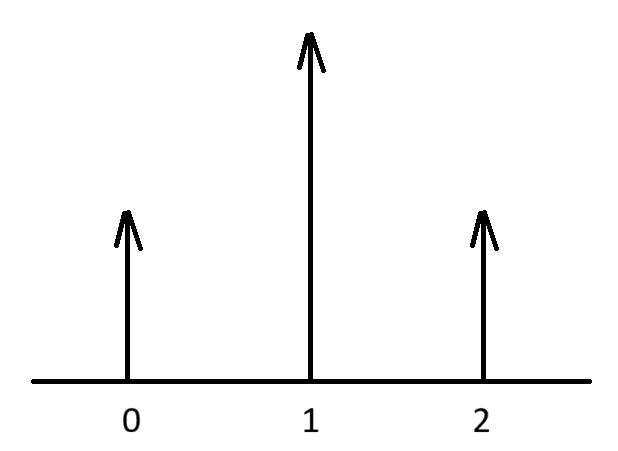
\includegraphics[width=0.5\linewidth]{Распределение 2 монет.png}
    \end{figure}
\end{example}

\begin{example}
    Так как схема Бернулли нам ещё встретится и не раз, то введём специальное обозначение для случайной величины, 
    которая отражает количество успехов в $n$ испытаниях Бернулли, и сразу запишем таблицу распределения:
    \renewcommand{\arraystretch}{2.2}
    \begin{table}[h]
    \centering
    \begin{tabular}{|*{7}{>{\centering\arraybackslash}m{2cm}|}}
    \hline
    $\beta_n^p$      & $0$ & $1$ & $\ldots$ & $k$ & $\ldots$ & $n$ \\
    \hline
    $P(\beta_n^p)$   & $q^n$ & $n p q^{n-1}$ & $\ldots$ & $\displaystyle \binom{n}{k} p^k q^{n-k}$ & $\ldots$ & $p^n$ \\
    \hline
    \end{tabular}
    \end{table} \leavevmode
    \\
    Диаграмма распределения будет выглядеть как ёжик (диграмма из примера 2.1, но и вправо, и влево имеем больше нисходящих стрелок). 
    Причём этот ёжик будет симметричным, если $p = q$. Если же равенство не достигается, то вершина его будет смещена в одну из сторон. \\ \\
    Стоит отметить, что размерность $\Omega$ оказалась сильно меньше размерности $\mathbb{X}$. Это наталкивает нас на мысль, что иногда 
    можно рассматривать какое-то $\mathbb{X}$, полученное из соображений здравого смысла, а не копаться в микроскопическом описании.
\end{example}

\begin{remark}
    Почему-то часто студенты валятся на следующем вопросе: 
    ``Как нам посчитать вероятность того, что $\xi$ примет значение из $A \subseteq \mathbb{X}$?''. Ответ:
    \[P(\xi \in A) \ = \sum_{k: \ x_k \in A} P_{\xi} (k)\]
    Забавно, что в силу упорядоченности иксов для подсчёта $P(\xi \geq b)$ 
    нам достаточно просто найти в таблице первый $x$, который не меньше $b$ и сложить все вероятности от него и вправо.
\end{remark}

\begin{example}
    Кидаем симметричную монету до выпадения герба. Пусть $\xi$ --- количество бросков. Тогда даже не будем рассматривать $\Omega$, а сразу 
    перейдём к $\mathbb{X} = \{1, 2, 3, \ldots, k, \ldots\}$. Таблица распределения для $\xi$ будет выглядеть так:
    \renewcommand{\arraystretch}{2.2}
    \begin{table}[h]
    \centering
    \begin{tabular}{|*{6}{>{\centering\arraybackslash}m{2cm}|}}
    \hline
    $x_i$           & $1$ & $2$ & $\ldots$ & $k$ & $\ldots$ \\
    \hline
    $P_{\xi} (i)$   & $\displaystyle \frac{1}{2}$ & $\displaystyle \frac{1}{4}$ & $\ldots$ & $\displaystyle \frac{1}{2^k}$ & $\ldots$ \\
    \hline
    \end{tabular}
    \end{table} \leavevmode
    \\
    Как раз получили пример, когда случайная величина $\xi$ имеет счётное число значений.
\end{example}

\section{Математическое ожидание случайной величины}

\begin{definition}
    \textbf{Математическое ожидание случайной величины} $\xi$ определим как
    \[E(\xi) := \sum_{i = 1}^{N(\Omega)} p_i \cdot \xi(\omega_i) = \sum_{k = 1}^{m} P_{\xi}(k) \cdot x_k\]
    Если $N(\Omega) = +\infty$, то $E(\xi)$ существует, если ряд сходится абсолютно. В случае с $m = +\infty$ 
    та же самая ситуация.
\end{definition}

\begin{remark}
    Математическое ожидание когда-то давно было получено как число, к которому сходится среднее арифметическое 
    результатов эксперимента при огромных числах повторений независимо от условий эксперимента.
\end{remark}

\begin{proof}
    На самом деле нам необходимо доказать, что два определения совпадают. 
    Действительно, $\xi(\omega_i) \in \mathbb{X} \ \forall i \implies$ сгруппируем слагаемые левой суммы по значениям $x_k$ (в случае абсолютно сходящегося ряда перестановки также уместны):
    \[\sum_{i = 1}^{N(\Omega)} p_i \cdot \xi(\omega_i) = \sum_{k = 1}^{m} \left(x_k \sum_{i: \xi(\omega_i) = x_k} p_i\right) = \sum_{k = 1}^{m} P_{\xi}(k) \cdot x_k\]
\end{proof}

\begin{remark}
    По-хорошему левое выражение больше похоже на определение, а правое --- на вычислительную формулу. 
    Поэтому на практике чаще всего используют именно правую часть, но левая ещё поможет вам в доказательствах.
\end{remark} \leavevmode
\\
Теперь посчитаем мат. ожидание случайных величин из примеров выше:
\newpage
\begin{example}
    Из примера 2.1: \\
    \renewcommand{\arraystretch}{2.2}
    \begin{table}[h]
    \centering
    \begin{tabular}{|*{4}{>{\centering\arraybackslash}m{2cm}|}}
    \hline
    $x_i$            & $0$ & $1$ & $2$ \\
    \hline
    $P_{\xi} (i)$   & $\displaystyle \frac{1}{4}$ & $\displaystyle \frac{1}{2}$ & $\displaystyle \frac{1}{4}$ \\
    \hline
    \end{tabular}
    \end{table}
    \[E(\xi) = 0 \cdot \frac{1}{4} + 1 \cdot \frac{1}{2} + 2 \cdot \frac{1}{4} = 1\]
\end{example}

\begin{example}
    Из примера 2.2: \\
    \renewcommand{\arraystretch}{2.2}
    \begin{table}[h]
    \centering
    \begin{tabular}{|*{7}{>{\centering\arraybackslash}m{2cm}|}}
    \hline
    $\beta_n^p$      & $0$ & $1$ & $\ldots$ & $k$ & $\ldots$ & $n$ \\
    \hline
    $P(\beta_n^p)$   & $q^n$ & $n p q^{n-1}$ & $\ldots$ & $\displaystyle \binom{n}{k} p^k q^{n-k}$ & $\ldots$ & $p^n$ \\
    \hline
    \end{tabular}
    \end{table}
    \[E(\xi) = \sum_{k = 0}^{n} k \binom{n}{k} p^k q^{n-k} = np\]
\end{example}

\begin{example}
    Из примера 2.3: \\
    \renewcommand{\arraystretch}{2.2}
    \begin{table}[h]
    \centering
    \begin{tabular}{|*{6}{>{\centering\arraybackslash}m{2cm}|}}
    \hline
    $x_i$           & $1$ & $2$ & $\ldots$ & $k$ & $\ldots$ \\
    \hline
    $P_{\xi} (i)$   & $\displaystyle \frac{1}{2}$ & $\displaystyle \frac{1}{4}$ & $\ldots$ & $\displaystyle \frac{1}{2^k}$ & $\ldots$ \\
    \hline
    \end{tabular}
    \end{table}
    \[E(\xi) = \sum_{k = 1}^{\infty} k \cdot \frac{1}{2^k} = 2\]
\end{example}

\section{А техи всё задерживаются...}

\begin{figure}[H]
    \centering
    
\includegraphics[width=1\linewidth]{Майя.jpg}
\end{figure}


\end{document}